\begin{satz}
Sei $f\in C^1\left(V,\mathbb{R}^{n-d}\right)$ mit $V$ offen und $c\in\mathbb{R}^{n-d}$ ein regulärer Wert von $f$. Dann ist die Niveaumenge $M\coloneqq\{v\in V \ | \ f(u)=c\}$ eine d-dimensionale Mannigfaltigkeit, für die gilt:
\begin{eqnarray*}
T_uM &=&\{v\in\mathbb{R}^n \ | \ f'(u)v=0\} \ \ \left(=\ker f'(u)\right) \ \ \forall u\in M \\
N_uM&=&\{w\in\mathbb{R}^n \ | \ w=f'(u)^Tv, v\in\mathbb{R}^{n-d}\} \ \ \forall u\in M 
\end{eqnarray*}
Das heißt also, die Spalten von $f'(u)^T$ bilden eines Basis des Normalenraums von $M$.
\end{satz}

\begin{beispiel}
Sei $f=\begin{pmatrix}
f_1 \\ f_2
\end{pmatrix}\in C^1\left(\mathbb{R}^3,\mathbb{R}^2\right)$ und $0\in\mathbb{R}^2$ ein regulärer Wert von $f$. Dann ist
\begin{equation*}
M:=\{u\in\mathbb{R}^3 \ | \underbrace{\ f_1(u)=0, \ f_2(u)=0}_{\text{Schnitt \ zweier \ Flächen}}\}
\end{equation*}
eine 1-dimensionale Mannigfaltigkeit. Dann steht der Gradient $f'_i(u)^T$ senkrecht auf $\{f_i=0\}$. $f'_1(u)^T$ und $f'_2(u)^T$ sind also Normalen zu $M$ in $u$.\\
\begin{center}
	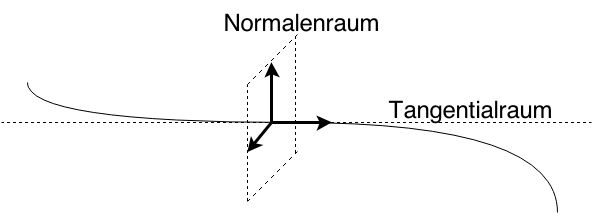
\includegraphics[scale=0.5]{pictures/003-01.png}
\end{center}
$v$ ist hier die Tangente, da $\scap{f'_i(u)^T}{v}=0$ ist (für $i=1,2$).
\end{beispiel}

\begin{proof}
Wir wissen bereits, dass $M$ eine Mannigfaltigkeit ist. Wählen wir nun die $C^1$-Kurve $\gamma$ auf $M$ mit $\gamma(0)=u$ und $\gamma'(0)=v$, so sehen wir, dass $f(\gamma(t))=c \ \forall t$ ist. $f'(u)$ steht senkrecht auf $v$ (also $\scap{f'(u)}{v}=0$) und da $\rang f'(u)=d$ ist, muss $\dim \ker f'(u)=d$ sein. Damit ist die Behauptung für $T_uM$ (wegen $\dim T_uM)=d$) gezeigt.\\
Nun wählen wir $w=f'(u)^T\tilde{v}$ und $w\in T_uM$. Offenbar ist $\scap{w}{v}=\scap{\tilde{v}}{f'(u)v}=0$. Damit ist $w$ im Normalenraum $N_uM$. Da $\rang f'(u)^T=n-d$  und $\dim N_uM=n-d$, folgt die Behauptung.
\end{proof}

\begin{beispiel}
Wir betrachten $M\coloneqq\mathcal{O}(n)=\{A\in\mathbb{R}^{n\times n}\ |\ A^TA=id \}$. 
Es handelt sich dabei um eine $\frac{n(n-1)}{2}$-dimensionale Mannigfaltigkeit von Matritzen. 
Man nennt $\mathcal{O}$ auch \emph{Orthogonale Gruppe} oder \emph{Lie-Gruppe}. 
Sie bildet die Menge aller orthogonale Matrizen des $\mathbb{R}^{n\times n}$. 
Offenbar ist $id$ das neutrale Element der Gruppe. Der Tangentialraum an diesem Element wird auch \emph{Lie-Algebra} genannt:
\begin{equation*}
T_{id}M=\{B\in\mathbb{R}^{n\times n}\ |\ B+B^T=0\}
\end{equation*}
Dies ist die Menge der schiefsymetrischen Matrizen. Warum ist das so?\\
\linebreak
Sei $f:\mathbb{R}^{n\times n}\rightarrow\mathbb{R}_{sym}^{n\times n}$ mit $f(A)=A^TA$ eine stetig differenzierbare Funktion mit $f'(A)B=A^TB+B^TA$ ($\forall B\in\mathbb{R}^{n\times n}$). Letzterer Ausdruck ist ebenfalls eine symetrische Matrix. 
$id$ ist ein regulärer Wert, denn sei $f(A)=id$ und $S\in\mathbb{R}_{sym}^{n\times n}$. $f'(A)B=S$ hat die Lösung $B=\frac{1}{2}AS$, denn $\frac{1}{2}A^TAS+\frac{1}{2}SA^TA=\frac{1}{2}S+\frac{1}{2}S=S$.
Letzteres hätte man auch in der Grundschule herausbekommen!\\
Aus vorheriger Überlegung folgt, dass $f'(A)$ vollen Rang hat. Aus Satz 4 wissen wir nun, dass die Dimension der Mannigfaltigkeit beträgt:
\begin{equation*}
d=\dim\mathbb{R}^{n\times n}-\dim\mathbb{R}_{sym}^{n\times n}=n^2-\frac{n(n+1)}{2}=\frac{n(n-1)}{2}
\end{equation*}
Satz 7 gewährleistet nun, dass
\begin{equation*}
T_{id}M=\{B\in\mathbb{R}^{n\times n} \ | \ id^TB+B^Tid=0\}
\end{equation*}
\end{beispiel}

\begin{definition}[Hyperflächen und Einheitsnormalenfelder]
Eine $(n-d)$-dimensionale Mannigfaltigkeit $M\subset\mathbb{R}^n$ heißt auch \textbf{Hyperfläche}. Die stetige Abbildung
\begin{equation*}
\nu:M\rightarrow\mathbb{R}^{n}
\end{equation*} 
heißt dann \textbf{Einheitsnormalenfeld}, falls 
\begin{equation*}
\nu(u)\in N_uM\ \mathrm{und\ } ||\nu(u)||=1 \ \ \forall u\in M
\end{equation*}
\begin{center}
	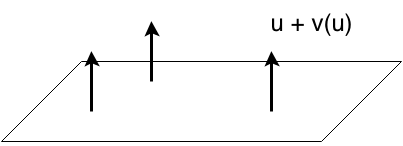
\includegraphics[scale=0.5]{pictures/003-02.png}
\end{center}
\end{definition}

\begin{lemma}
Ist $M\subset\mathbb{R}^n$ eine zusammenhängende Hyperflääche, so existiert entweder \emph{kein} oder \emph{genau zwei} Einheitsnormalenfelder. 
\end{lemma}

\begin{proof}
Als Vorbetrachtung lässt sich sagen, dass wenn $\nu$ ein Einheitsnormalenfeld ist, auch $-\nu$ eins sein muss.\\
Nehmen wir nun an, es gäbe zwei verschiedene Einheitsnormalenfelder $\nu$ und $\tilde{\nu}$. 
Wir können ausnutzen, dass die beiden Felder normiert sind und stellen sofort fest, da $\dim N_uM=1$ ist, dass das Skalarprodukt der beiden nur
\begin{equation*}
s(u)\coloneqq\scap{\nu(u)}{\tilde{\nu}(u)}=\pm 1
\end{equation*}
sein kann. Wir können nun eine weitere wichtige Eigenschaft von $s$ und $M$ ausnutzen.
Da $M$ zusammenhängend und $s$ stetig auf $M$ ist, lässt sich der Zwischenwertsatz zu Hilfe nehmen, 
der uns liefert, dass $s$ für alle $u$ konstant sein \emph{muss}, nämlich entweder $s(u)=1$ oder $s(u)=-1$.
Damit kann $\tilde{\nu}$ nur entweder gleich $\nu$ oder gleich $-\nu$ sein.
\end{proof}

\begin{beispiel}[Möbiusband]
Das wohlbekannte Möbiusband besitzt \emph{kein} Einheitsnormalenfeld.\\
\textbf{grafk fehlt.} 
\end{beispiel}

\begin{beispiel}
Wir betrachten die Konstruktion von Einheitsnormalenfeldern für Hyperflächen $M\coloneqq \{f=0\}$.
Sei $f\in C^1\left(V,\mathbb{R}\right)$ mit $V$ offen und $0$ ein regulärer Wert von $f$. 
Wir können leicht ein Einheitsnormalenfeld definieren und wählen
\begin{equation*}
\nu(u)\coloneqq\frac{f'(u)}{||f'(u)||}
\end{equation*}
\end{beispiel}

Wir wollen nun im folgenden weitere Operationen auf Mannigfaltigkeiten untersuchen.
Im $\mathbb{R}^n$ ist uns das Kreuzprodukt $...\times...$ wohlbekannt.
Es ist zweckmäßig diesen Begriff auf beliege Dimensionen zu verallgemeinern.
\begin{definition}[Äußeres Produkt]
Nehmen wir uns die Vektoren $a_1,a_2,...,a_{n-1}\in\mathbb{R}^n$ und schreiben sie einfach als Spaltenvektoren hintereinander in eine Matrix:
\begin{equation*}
A\coloneqq(a_1|a_2|...|a_{n-1})\in\mathbb{R}^{n\times(n-1)}
\end{equation*}
Wir entfernen nun aus dieser die $k$-te Zeile und nennen sie dann $A_k\in\mathbb{R}^{(n-1)\times(n-1)}$. 
Den Ausdruck
\begin{equation*}
a_1\wedge a_2\wedge...\wedge a_{n-1}\coloneqq\alpha=\begin{pmatrix}
\alpha_1 \\ \alpha_2 \\ \vdots \\ \alpha_k
\end{pmatrix}
\end{equation*}
nennen wir \textbf{äußeres Produkt} von $a_1,a_2,...,a_{n-1}$, wobei
\begin{equation*}
\alpha_k=(-1)^{k-1}\cdot\det A_k
\end{equation*}
\end{definition}
Wir können sofort einige interessante Eigenschaften ablesen, die uns an das bekannte Kreuzprodukt erinnern:
\begin{enumerate}
\item $\alpha$ steht senkrecht auf allen $a_1,a_2,...,a_{n-1}$.
\item Das \emph{Volumen} des von $a_1,a_2,...,a_{n-1}$ aufgespannten Parallelotops  entspricht gerade der Norm $||\alpha||$ des äußeres Produkts.
\end{enumerate}

\begin{beispiel}
Die eben untersuchten Eigenschaften bringen uns dazu, im $\mathbb{R}^3$ das äußerde Produkt mit dem Kreuzprodukt zu identifizieren.
\begin{equation*}
\alpha_1\wedge\alpha_2\equiv\alpha_1\times\alpha_2 \ \ \ \ \ \text{für\ } n=3
\end{equation*}
\end{beispiel}

\begin{lemma}
Sind $b, a_1,a_2,...,a_{n-1}\in\mathbb{R}^n$, so ist
\begin{equation}
\scap{b}{a_1\wedge a_2\wedge...\wedge a_{n-1}}=\det (b | a_1|a_2|...|a_{n-1})
\end{equation}
wobei
\begin{equation*}
a_1\wedge a_2\wedge...\wedge a_{n-1} \ \bot a_i
\end{equation*}
und
\begin{equation*}
a_1\wedge a_2\wedge...\wedge a_{n-1} \ \ \ \ \ \left\{\begin{matrix}
=0 \ \ \text{falls\ }a_i\ \text{linear abhängig} \\
\ \ \ \ \ \neq 0 \ \ \text{falls\ }a_i\ \text{linear unabhängig}
\end{matrix}\right.
\end{equation*}
\end{lemma}

\begin{proof}
Wir können die Determinante in (29.4) nach der 1. Spalte $b$ entwickeln. Aus $b=a_i$ folgen die Bedingungen.
\end{proof}

\begin{beispiel}
Konstruieren wir ein Einheitsnormalenfeld mittels der Parametrisierung $\varphi:V\subset\mathbb{R}^{n-1}\rightarrow\mathbb{R}^n$ mit $V$ offen. 
$M=\{\varphi(v)\}$ sei die entsprechende Hyperfläche. Nach Satz 6 wissen wir, dass $\pdiff{}{x_j}\varphi(x)$ für alle $x$ und für alle $j=1,2,...,n-1$ im Tangentialraum $T_{\varphi(x)}M$ liegt. Wir erkennen außerdem, dass 
\begin{equation*}
N(x)\coloneqq\varphi_{x_1}(x)\wedge\varphi_{x_2}(x)\wedge ... \wedge\varphi_{x_{n-1}}
\end{equation*}
in $N_{\varphi(x)}M$ liegt und können damit
\begin{equation*}
\nu(x)\coloneqq\frac{N(x)}{||N(x)||}
\end{equation*}
als Einheitsnormalenfeld von $M$ wählen. Man beachte, dass $\varphi'(x)$ für alle $x$ regulär ist!
\end{beispiel}
Wir kommen zum Abschluss dieses Kapitels. Wir haben uns mit Mannigfaltigkeiten und ihren Eigenschaften beschäftigt. Als nächstes möchten wir die Integration auf ihnen untersuchen, beschränken uns dabei jedoch noch auf Kartengebiete.

\section{Integration auf Kartengebieten}
\setcounter{equation}{0}     %Quick fix for equation-counters not resetting with section
Wir stellen uns zunächst die interessante Frage, wie man den Oberflächeninhalt beziehungsweise das d-dimensionale Äquivalent dazu von einer Mannigfaltigkeit bestimmen kann. 
Die Idee wäre natürlich, wie etwa bei der Integration über $\mathbb{R}$, sie durch \emph{ebene} Mannigfaltigkeiten (etwa mit Dreiecken) stückweise zu approximieren.\\
\begin{center}
	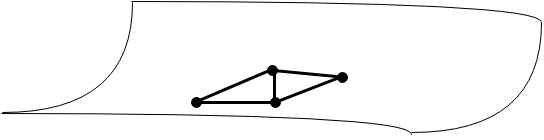
\includegraphics[scale=0.5]{pictures/003-03.png}
\end{center}
\begin{equation*}
\textbf{Fläche}(M)=\sup \sum\limits_\Delta \textbf{Dreiecksflächen}
\end{equation*}
Wir stellen jedoch mit großem Entsetzen schnell fest, dass diese Methode nur für Kurven ($d=1$) funktioniert.\\
\begin{center}
	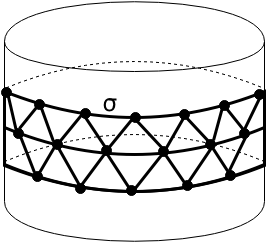
\includegraphics[scale=0.5]{pictures/003-04.png}
\end{center}
Schauen wir uns zum Beispiel eine Zylinderfläche $M\subset\mathbb{R}^3$ an. 
Lassen wir die Feinheit $\sigma$ beliebig klein werden - heute ist ja schließlich alles nano! - so wachsen die Dreiecksflächen immer weiter, 
bis die Fläche von $M$ über alle Grenzen hinaus wächst. Wir müssen uns also wohl sofort wieder von dieser Methode verabschieden.\\
\begin{center}
	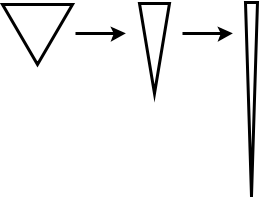
\includegraphics[scale=0.5]{pictures/003-05.png}
\end{center}
\emph{Über dieses Dilemma nachlesen kann man übrigens in Hildebrand, Analysis 2 unter ''Schwartz'scher Stiefel''.}\\
\linebreak
Versuchen wir also etwas neues (für $d=2$) zu finden. Wir nehmen hierzu tangentionale Parallelogramme (äußere Approximation).
$\varphi'(x):\mathbb{R}^d\rightarrow\mathbb{R}^n$ ist linear. Die Methode gestaltet sich also zu
\begin{equation*}
\textbf{Fläche}(M)=\lim\limits_{\sigma\rightarrow 0}\left(\sum\textbf{Fläche\ }\varphi'(x_j)(Q)\right)
\end{equation*}
\begin{center}
	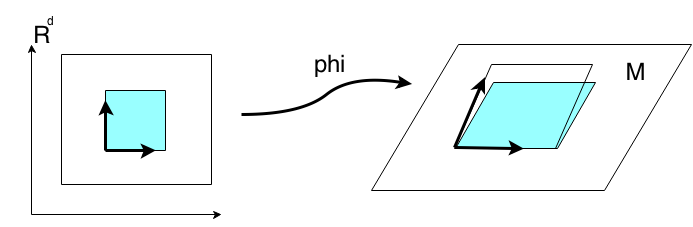
\includegraphics[scale=0.5]{pictures/003-06.png}
\end{center}